\documentclass{sigplanconf}

\usepackage{amsmath}
\usepackage[utf8]{inputenc}
\usepackage{graphicx}

\begin{document}
\newcommand{\fig}[1]{(fig. \ref{fig:#1})}
\newcommand{\figg}[2]{(fig. \ref{fig:#1}, \ref{fig:#2})}

\conferenceinfo{ESUG '05}{August 22nd 2011, Edimburgh.} 
\copyrightyear{2011} 
\copyrightdata{[to be supplied]} 

\titlebanner{banner above paper title}        % These are ignored unless
\preprintfooter{short description of paper}   % 'preprint' option specified.

\title{A programming environment supporting an instance-based introduction to OOP}
\subtitle{}

\authorinfo{Carla Griggio$^\dagger$ 
			\and Germán Leiva$^{\dagger\ddagger}$ 
			\and Guillermo Polito$^{\dagger\ddagger}$  
			\and Gisela Decuzzi$^\dagger$  
			\and Nicolás Passerini$^{\dagger\ddagger}$ }
           {$^\dagger$Universidad Tecnológica Nacional (UTN) -- Argentina 
           \and $^\ddagger$Universidad Nacional de Quilmes (UNQ) -- Argentina}
           {\{carla.griggio $|$ giseladecuzzi $|$ leivagerman $|$ guillermopolito $|$ npasserini\}@gmail.com}
% \authorinfo{}	
%            {Universidad Tecnológica Nacional \\ Universidad Nacional de Quilmes \\ Argentina}
%            {\{leivagerman|guillermopolito|\\npasserini\}@gmail.com}

\maketitle

\begin{abstract}
This paper describes the features that a programming environment should have in order to help learning the object-oriented programming (OOP) paradigm and let students get the skills needed to build software using objects very quickly. This proposal is centered on providing graphical tools to help understand the concepts of the paradigm and let students create objects before they are presented the class concept \cite{Utti10}. The object, message and reference concepts are considered of primary importance during the teaching process, allowing quick acquisition of both theory and practice of concepts such as delegation, polymorphism and composition \cite{Lomb07}.
Additionally, a current implementation of the proposed software and the experience gained so far using it for teaching at universities and work trainings. Finally, we describe possible extensions to the proposed software that are currently under study.
\end{abstract}

\category{K.3.2}{Computer and Information Science Education}{computer science education, information systems education}
\category{D.3.2}{Language Classificationss}{object-oriented languages}
\category{D.3.3}{Language Constructs and Features}{classes and objects, inheritance, polymorphism}

\terms
Experimentation, Human Factors, Languages

\keywords
Educational programming environments, object-oriented programming, teaching methodologies, prototype-based, explicit garbage collection, objects visualization

\section{Introduction}

Frequently, in introductory courses to OOP, students have prior experience in structured programming. 
This is often counter-productive when understanding some of the basic concepts of the OOP paradigm, such as the relationship between a class and its instances, the difference between object and reference, delegation and polymorphism \cite{Weir05}. In order to minimize this difficulty, a possible strategy is to postpone the introduction of the class concept. This reduces the set of concepts needed to build programs \cite{Lomb07}. 

Similiar difficulties appear in students who do not have prior knowledge in programming at the time of learning OOP, and specially in those cases it is convinient to bring down any complexity that a language might have in order to understand the ideas the paradigm proposes \cite{Vent04}.

To provide support to an introduction of OOP without working with the concept of class we believe it is necessary to have a programming environment in which the object and the message are the central concepts instead of defining classes and then instantiate them.
Moreover, it has to offer facilities to understand the concepts of environment, state and garbage collection.

\section{Proposed programming environment}

In this section we describe the features for a programming environment which helps our objectives, 
stating which common learning difficulties have to be prevented when introducing the OOP paradigm to students. 

\subsection{Multiple object environments - lessons}

In order to introduce the concept of object environment we propose using lessons: an object environment associated to a group of objects, the references pointing to them, a workspace to interact with them and an object diagram. Lessons should be independent from each other; none of the elements mentioned above should be shared between different lessons.

The use of lessons also aims to help students organize their work and let the teacher offer environments with pre-existing objects as scenarios for excercises.

\subsection{Defining and using objects}
We believe that a visual tool to create objects allows the student to build programs focusing on object use instead of object creation at the first stages of the learning process. We propose to work with a simplified prototype oriented environment \cite{Wilk02,Mads96}, where the objects contain their own methods without the need of classes; and the creation of objects, attributes and methods is performed through a visual approach. This simplified object-oriented programming environment allows students to build programs in a very early stage of the course with many collaborating objects and making use of polymorphism.

Since the proposed environment lacks the concepts of classes or inheritance, the
reuse of code is achieved by cloning objects. The cloning mechanism is simpler
than those found in Self \cite{Unga07} or Javascript \cite{Wilk02}. In those languages, tipically a
prototypical object is divided in two parts, one containing the behavioral
slots, which will be shared as a \textit{parent object} among all the cloned
objects, and another part containing the ``state'' slots, which must be cloned every time a new object is created. In our proposal, the same object servers the two purposes: 
\begin{itemize}
\item the new object has the same internal structure as the original one. 
\item the new object has the cloned one as delegate. This means that the new
object \textit{inherites} all of the behaviour of the original one, but also it can \textit{override} its behaviour by defining methods with the same name.
\end{itemize}	
This simplified prototype approach enables code sharing mechanisms and facilitate the introduction of classes and inheritance in a later stage of the course based on a more classical view of the object-oriented paradigm.

To improve the student’s programming experience, the environment should provide ready-to-use basic prototype objects such as numbers, booleans, collections and dates; in order to do more complex exercises the environment could also include networking, persistency and graphical user interface objects.

\subsection{Objects and References}
Students often confuse objects and references, believing they are the same. In order to make the difference more clear, our proposal is to separate the addition of a new object to the environment in two steps. The first step is to create a \textit{nameless} object. In the second step we give the created object a name, by associating a reference to it; this can be done by creating a new reference or by redirecting an existing reference. The association between the object and the reference could be done graphically using the object diagram. 

This explicit separation between the created object and a reference pointing to it, improves the understanding of the difference between both concepts. Once established that difference, assignments could be used by the students without fear.

\subsection{Object Diagram}

A lesson should provide its own object diagram, where one can appreciate
visually the relationship between living objects in that lesson’s environment.
This tool makes it easier to get a clearer distinction between the concept of object and reference, and helps to comprehend the state of the environment of the lesson at a given moment. 

When the student interacts with the objects from a workspace, the diagram shows the state changes while the program executes. This provides a live vision of what happens in the object environment after each message-send. 

The visual representation of the objects and references in the environment and the ability to folow their changes along with the program execution improves the understanding of some important concepts of the paradigm: like references and object identity.

\subsection{Garbage Collection}

Students usually want to erase an object from their system and find it odd not to have an explicit way to do so, e.g. sending a message delete, free or dealloc.

In order to help understanding how the garbage collector works \cite{Hert05}, we propose using an explicit mechanism of garbage collection to clarify the conditions that make an object likely to be collected. This way, students are able to observe which objects can be erased and give the explicit order to do so.

The proposed approach is centered on using the object diagram to illustrate the different stages an object goes through until it is collected. Once an object is not referenced by any other object, it should not disappear of the environment automatically, and in the object diagram it should appear isolated from the rest of the lesson's object graph, standing out as an object likely to be collected. This way, the student can see clearly that there are no references pointing to it. A garbage collection can be explicitly run at any time removing every unreferenced object from the lesson's environment and the object diagram as well.

\section{Implementations}

The first implementation of a tool based on the proposed style was an add-on for the Dolphin Smalltalk\footnote{Object Arts Dolphin Smalltalk: http://www.object-arts.com/} environment which allowed the creation of objects without using classes and had a workspace to interact with them \cite{Lomb07}.  We used that first implementation to put in practice the idea of delaying the introduction of the class concept, and it was also useful as a model for the next implementations.

\bigskip
Nowadays, there is a new version of that tool built on top of Pharo Smalltalk\footnote{Pharo Smalltalk: http://www.pharo-project.org/} named LOOP  (Learning Object Oriented Programming) implementing the first versions of the features described above \cite{Lomb07}.

The main menu of LOOP is a Lesson Browser \fig{lessonBrowser}, where lessons can be created, opened, deleted, exported to a file for sharing and imported back in the Pharo image. Exporting and importing a lesson is very useful for the teacher to evaluate excercises done by the students and also give them prebuilt lessons.
\begin{figure}[h]
 \centering
 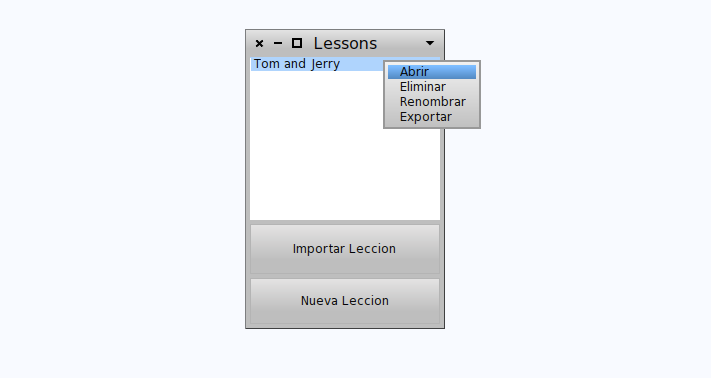
\includegraphics[scale=.35]{./images/lessonBrowser.png}
 \caption{Lesson Browser}
 \label{fig:lessonBrowser}
\end{figure}

To create objects and references inside a lesson, the user has to use the object browser, which shows every reference and object created in the lesson environment. Selecting a reference from the menu brings up the object inspection window for the object that it points to, where the user can browse and define its attributes and methods \fig{objectBrowser}. 
\begin{figure}[h]
 \centering
 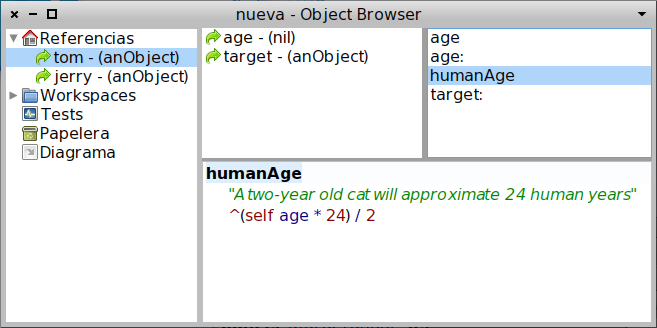
\includegraphics[scale=.35]{./images/objectBrowser.png}
 \caption{Object Browser}
 \label{fig:objectBrowser}
\end{figure}

A live object diagram shows the state of a lesson’s environment and it is updated after every action that affects the environment state, i.e. addition or deletion of attributes of an object, message sends with side effects, creation of new objects, garbage collection, etc. \fig{workspace}.
\begin{figure}[h]
 \centering
 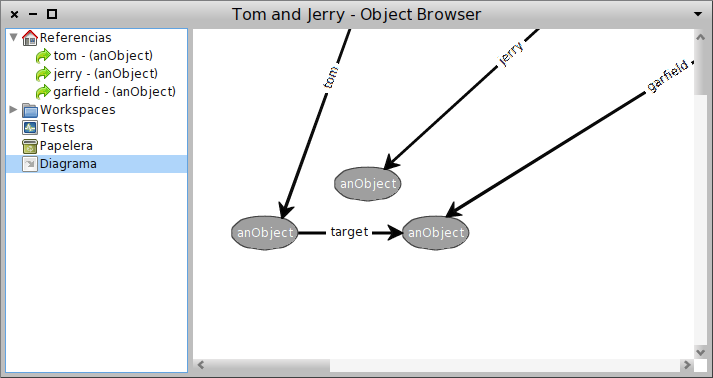
\includegraphics[scale=.35]{./images/workspace.png}
 \caption{Interacting with objects from a workspace}
 \label{fig:workspace}
\end{figure}

The user can define many workspaces with different scenarios of interaction with the objects within the lesson \fig{objectDiagram}. 
\begin{figure}[h]
 \centering
 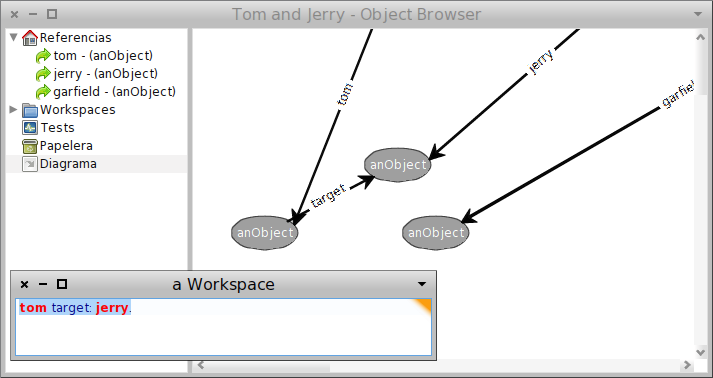
\includegraphics[scale=.35]{./images/objectDiagram.png}
 \caption{Object Diagram}
 \label{fig:objectDiagram}
\end{figure}

The explicit garbage collection mechanism is illustrated with a Garbage Bin metaphore. Candidates for collection can be easily found in the object diagram because they would have no arrows pointing at them, and the Garbage Bin lists those same unreferenced objects \fig{deletingAReference}. When the Garbage Bin is emptied, those unreferenced objects are deleted from the environment and dissappear from the object diagram \figg{beforeGarbageCollection} {afterGarbageCollection}.
\begin{figure}[h]
 \centering
 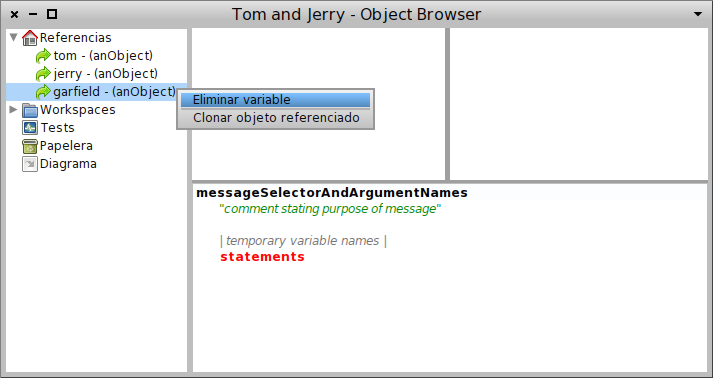
\includegraphics[scale=.35]{./images/deletingAReference.png}
 \caption{Deleting a reference}
 \label{fig:deletingAReference}
\end{figure}
\begin{figure}[h]
 \centering
 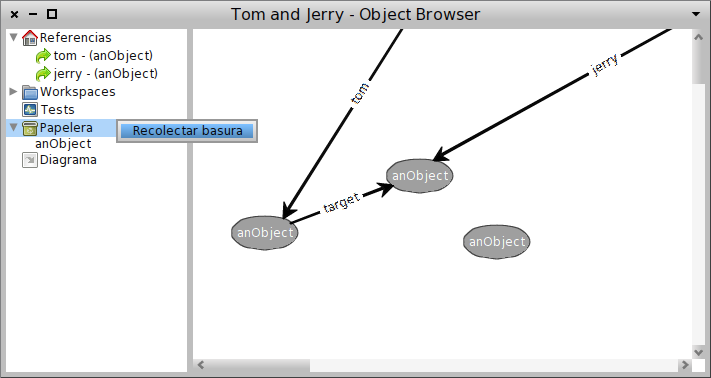
\includegraphics[scale=.35]{./images/beforeGarbageCollection.png}
 \caption{Object environment before garbage collection}
 \label{fig:beforeGarbageCollection}
\end{figure}
\begin{figure}[h]
 \centering
 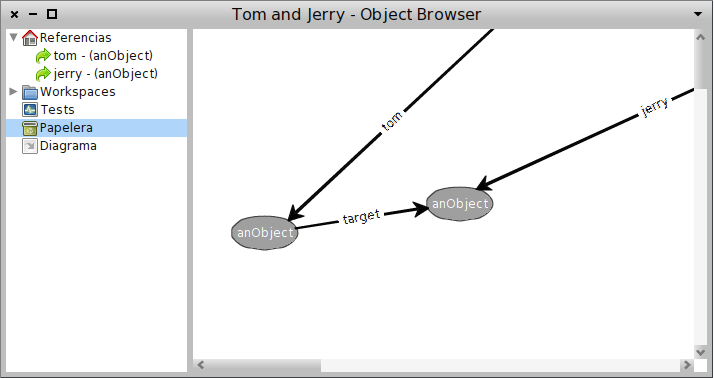
\includegraphics[scale=.35]{./images/afterGarbageCollection.png}
 \caption{Object environment after garbage collection}
 \label{fig:afterGarbageCollection}
\end{figure}

\section{Experiences}

LOOP was used in university courses and job trainings to put in practice the concepts of polymorfism, object composition and delegation from the start.  Afterwards, the concepts tought in the class was introduced as an alternative to build objects and share and extend their behavior without difficulties.

\bigskip
In UTN and UNQ object oriented courses where LOOP was used the students were already experienced with structured programming.  The visual environment helped them to face the learning process without trying to just match their previous knowledge.

In object oriented job training for technologies like Smalltalk or Java, most of the trainees had few or no programming experience. Those courses demanded high quality training in a short time. Using LOOP intensively in the first lessons to introduce the paradigm, the transition to an specific programming language was faster than in previous courses. Also, the aspirants who used LOOP, showed a higher learning curve for other object-oriented technologies.

\section{Conclusions}

Our experience using LOOP shows that students learn the object oriented programming paradigm more easily when we incorporate a programming environment offering visual tools for creating objects and interacting with them. Also, defining our own programming environment, allows us to select the programming concepts we want to introduce at each step of the learning process, providing an excellent ground for a gradual introduction of those concepts. The programming environment proves to be very useful for students, with or without previous programming knowledge, because it allows them to focus on the most important concepts of the programming paradigm, avoiding technology-specific distracting elements. A solid knowledge of those concepts facilitates a later transition to any other object-oriented programming language.

\section{Further work}

The current implementation of LOOP is based on Smalltalk and the syntax used when programming is the syntax of the Smalltalk language. We think this syntax is the best choice for an introductory course, because of its simplicity and is resemblance of the natural language. Also it is meant for courses that, after an introduction based on LOOP, can continue learning object-oriented programming in a real Smalltalk environment. Nevertheless, we consider that a future implementation of LOOP should include a configurable syntax, allowing the teacher to choose the most similar option to that of the language he is planing to use in the later stages of the course. For example, if the course is going to continue using the Java language, a C-like syntax could be considered for being used on LOOP. This would allow us to take the most of LOOP also in courses based on other languages different from Smalltalk. Besides, the tool could allow the teacher to configure its own syntax.

We also want to include a configurable type system. We think that explicit type definitions take the focus away from the most important concepts of the paradigm and should be preferably avoided in introductory courses. Nevertheless, since many object-oriented languages make heavy use of static type-systems with explicit type definitions, a configurable type-system should also be considered.

The current implementation of LOOP offers a limited support for developing unit tests [Figure 7]. This part of the tool should be improved in order to facilitate the use of test-driven development (TDD) from the begining of the course. Since the nature of LOOP programming environment imposes some specific difficulties to build tests without side-effect, a concrete implementation of TDD inside of LOOP is still to be analyzed in depth.

We also consider improving both appearance and functionality of the graphical diagrams of LOOP [Figure 3]. Object diagrams should be interactive, allowing the creation of new objects or sending messages from the diagram itself, as an alternative to the workspace and the reference-panel [Figure 2]. Also, sequence and collaboration diagrams would be useful for the comprehension of the dynamic relationships between objects. This kind of diagrams could be inferred from the evaluation of any piece of code, even the execution of tests.

Another subject of research is a ``debugger'' for the tool \cite{Benn10}. We think that a live and powerful debugger \textit{à la Smalltalk} is a rich tool for the understanding of the whole environment behaviour. 
After a message is sent, a debugger view can be used like a video player, with play, forward and  backward buttons to navigate the message stack and see how the state changes after each message send in the object diagram.

Finally, there are some improvements to be made to the user interface, such as shortcuts, code completion, improved menues or internationalization. Currently the tool is only available in spanish, we want to make it configurable to add more languages as necessary.

\acks

Carlos Lombardi and Leonardo Cesario collaborated in the first implementation of the programming environment. Also, many of the teachers and students of the subjects of \textit{Programming Paradigms} at UTN and \textit{Computers II} at UNQ gave us great help by testing our tools, reporting bugs and proposing new ideas. Gabriela Arévalo, Victoria Griggio and Débora Fortini helped us in the writing of this paper.

\nocite{Libe11,Mich00,Kouz07,Shan06,Shch95}
% We recommend abbrvnat bibliography style.

\bibliographystyle{abbrvnat}
%\bibliography{loop}

\begin{thebibliography}{}
\softraggedright

\providecommand{\natexlab}[1]{#1}
\providecommand{\url}[1]{\texttt{#1}}
\expandafter\ifx\csname urlstyle\endcsname\relax
  \providecommand{\doi}[1]{doi: #1}\else
  \providecommand{\doi}{doi: \begingroup \urlstyle{rm}\Url}\fi

\bibitem[Bennedsen and Schulte(2010)]{Benn10}
J.~Bennedsen and C.~Schulte.
\newblock Bluej visual debugger for learning the execution of object-oriented
  programs?
\newblock \emph{Trans. Comput. Educ.}, 10:\penalty0 8:1--8:22, June 2010.
\newblock ISSN 1946-6226.
\newblock \doi{http://doi.acm.org/10.1145/1789934.1789938}.
\newblock URL \url{http://doi.acm.org/10.1145/1789934.1789938}.

\bibitem[Hertz and Berger(2005)]{Hert05}
M.~Hertz and E.~D. Berger.
\newblock Quantifying the performance of garbage collection vs. explicit memory
  management.
\newblock In \emph{Proceedings of the 20th annual ACM SIGPLAN conference on
  Object-oriented programming, systems, languages, and applications}, OOPSLA
  '05, pages 313--326, New York, NY, USA, 2005. ACM.
\newblock ISBN 1-59593-031-0.
\newblock \doi{http://doi.acm.org/10.1145/1094811.1094836}.
\newblock URL \url{http://doi.acm.org/10.1145/1094811.1094836}.

\bibitem[Kouznetsova(2007)]{Kouz07}
S.~Kouznetsova.
\newblock Using bluej and blackjack to teach object-oriented design concepts in
  cs1.
\newblock \emph{J. Comput. Small Coll.}, 22:\penalty0 49--55, April 2007.
\newblock ISSN 1937-4771.
\newblock URL \url{http://portal.acm.org/citation.cfm?id=1229637.1229646}.

\bibitem[Liberman et~al.(2011)Liberman, Beeri, and Ben-David~Kolikant]{Libe11}
N.~Liberman, C.~Beeri, and Y.~Ben-David~Kolikant.
\newblock Difficulties in learning inheritance and polymorphism.
\newblock \emph{Trans. Comput. Educ.}, 11:\penalty0 4:1--4:23, February 2011.
\newblock ISSN 1946-6226.
\newblock \doi{http://doi.acm.org/1921607.1921611}.
\newblock URL \url{http://doi.acm.org/1921607.1921611}.

\bibitem[Lombardi et~al.(2007)Lombardi, Passerini, and Cesario]{Lomb07}
C.~Lombardi, N.~Passerini, and L.~Cesario.
\newblock Instances and classes in the introduction of object oriented
  programming.
\newblock \emph{Smalltalks 2007 -- Primera Conferencia Argentina de Smalltalk},
  2007.

\bibitem[Madsen(1996)]{Mads96}
O.~Madsen.
\newblock Strategic research directions in object-oriented programming.
\newblock \emph{ACM Comput. Surv.}, 28, December 1996.
\newblock ISSN 0360-0300.
\newblock \doi{http://doi.acm.org/10.1145/242224.242424}.
\newblock URL \url{http://doi.acm.org/10.1145/242224.242424}.

\bibitem[Michiels et~al.(2000)Michiels, Fern\'{a}ndez, B\"{o}rstler, and
  Prieto]{Mich00}
I.~Michiels, A.~Fern\'{a}ndez, J.~B\"{o}rstler, and M.~Prieto.
\newblock Tools and environments for understanding object-oriented concepts.
\newblock In \emph{Proceedings of the Workshops, Panels, and Posters on
  Object-Oriented Technology}, ECOOP '00, pages 65--77, London, UK, 2000.
  Springer-Verlag.
\newblock ISBN 3-540-41513-0.
\newblock URL \url{http://portal.acm.org/citation.cfm?id=646780.705783}.

\bibitem[Shanmugasundaram et~al.(2006)Shanmugasundaram, Juell, and
  Hill]{Shan06}
V.~Shanmugasundaram, P.~Juell, and C.~Hill.
\newblock Knowledge building using visualizations.
\newblock In \emph{Proceedings of the 11th annual SIGCSE conference on
  Innovation and technology in computer science education}, ITICSE '06, pages
  23--27, New York, NY, USA, 2006. ACM.
\newblock ISBN 1-59593-055-8.
\newblock \doi{http://doi.acm.org/10.1145/1140124.1140134}.
\newblock URL \url{http://doi.acm.org/10.1145/1140124.1140134}.

\bibitem[Shcherbina et~al.(1995)Shcherbina, Vortman, and Zodik]{Shch95}
V.~Shcherbina, P.~Vortman, and G.~Zodik.
\newblock A visual object-oriented development environment (voode).
\newblock In \emph{Proceedings of the 1995 conference of the Centre for
  Advanced Studies on Collaborative research}, CASCON '95, pages 57--. IBM
  Press, 1995.
\newblock URL \url{http://portal.acm.org/citation.cfm?id=781915.781972}.

\bibitem[Ungar and Smith(2007)]{Unga07}
D.~Ungar and R.~B. Smith.
\newblock Self.
\newblock In \emph{Proceedings of the third ACM SIGPLAN conference on History
  of programming languages}, HOPL III, pages 9--1--9--50, New York, NY, USA,
  2007. ACM.
\newblock ISBN 978-1-59593-766-7.
\newblock \doi{http://doi.acm.org/10.1145/1238844.1238853}.
\newblock URL \url{http://doi.acm.org/10.1145/1238844.1238853}.

\bibitem[Utting et~al.(2010)Utting, Cooper, K\"{o}lling, Maloney, and
  Resnick]{Utti10}
I.~Utting, S.~Cooper, M.~K\"{o}lling, J.~Maloney, and M.~Resnick.
\newblock Alice, greenfoot, and scratch -- a discussion.
\newblock \emph{Trans. Comput. Educ.}, 10:\penalty0 17:1--17:11, November 2010.
\newblock ISSN 1946-6226.
\newblock \doi{http://doi.acm.org/10.1145/1868358.1868364}.
\newblock URL \url{http://doi.acm.org/10.1145/1868358.1868364}.

\bibitem[Ventura and Ramamurthy(2004)]{Vent04}
P.~Ventura and B.~Ramamurthy.
\newblock Wanted: Cs1 students. no experience required.
\newblock In \emph{Proceedings of the 35th SIGCSE technical symposium on
  Computer science education}, SIGCSE '04, pages 240--244, New York, NY, USA,
  2004. ACM.
\newblock ISBN 1-58113-798-2.
\newblock \doi{http://doi.acm.org/10.1145/971300.971387}.
\newblock URL \url{http://doi.acm.org/10.1145/971300.971387}.

\bibitem[Weir et~al.(2005)Weir, Vilner, Mendes, and Nordstr\"{o}m]{Weir05}
G.~R.~S. Weir, T.~Vilner, A.~J. Mendes, and M.~Nordstr\"{o}m.
\newblock Difficulties teaching java in cs1 and how we aim to solve them.
\newblock In \emph{Proceedings of the 10th annual SIGCSE conference on
  Innovation and technology in computer science education}, ITiCSE '05, pages
  344--345, New York, NY, USA, 2005. ACM.
\newblock ISBN 1-59593-024-8.
\newblock \doi{http://doi.acm.org/10.1145/1067445.1067543}.
\newblock URL \url{http://doi.acm.org/10.1145/1067445.1067543}.

\bibitem[Wilkens(2002)]{Wilk02}
L.~Wilkens.
\newblock Objects with prototype-based mechanisms.
\newblock \emph{J. Comput. Small Coll.}, 17:\penalty0 131--140, February 2002.
\newblock ISSN 1937-4771.
\newblock URL \url{http://portal.acm.org/citation.cfm?id=772636.772659}.

\end{thebibliography}

\end{document}
